\subsection{Dataset description and generator} \label{subsec:dataset}
Recurrent Neural Network is a subclass of NN, proven effective in weather or stock prices forecasting.
This method learns by recognising a pattern within sequential data input, thus predicting the future outcome.
It makes the following approach applicable to almost any type of time series dependant problem~\cite{anton_battery_2013}.
Classical RNN consists primarily of three layers, represented in \mbox{Figure~\ref{fig:RNN-structure}}.
The two vectors or matrices define the Input and Output Layers.
The general description of a single input X and an output Y samples are represented by \mbox{Equations~\ref{eq:xy-matrix}}.
$V, I, T, SoC$ represent Voltage (V), Current (A), Temperature (\textdegree{}C) as input features, and percentage of State of Charge (between 0 and 1) as output.
All samples are equally time distributed, and the t represents the number of input time steps at a time.
\begin{figure}[htbp]
    \centering
    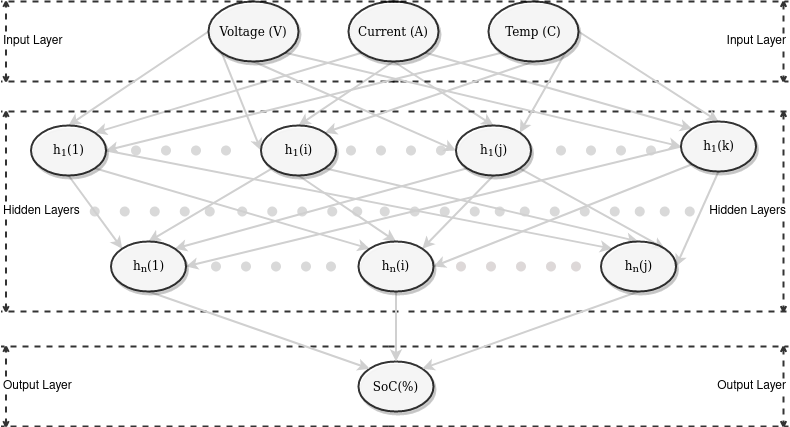
\includegraphics[width=\columnwidth]{II_Body/images/SoC-RNN.png}
    \caption{Universal structure of RNN for SoC estimation.}
    \label{fig:RNN-structure}
\end{figure}
\begin{equation}
    \textbf{X} \left (n  \right ) = 
    \begin{Bmatrix}
        V \left (0  \right ) & V \left (1  \right ) & ... & V \left (t  \right )\\ 
        I \left (0  \right ) & I \left (1  \right ) & ... & I \left (t  \right )\\ 
        T \left (0  \right ) & T \left (1  \right ) & ... & T \left (t  \right )\\
    \end{Bmatrix}
    \\ \textbf{Y} \left (n  \right ) = 
    \begin{Bmatrix}
        SoC \left (t  \right ) 
    \end{Bmatrix}
\label{eq:xy-matrix}
\end{equation}

%
%
For dataset generation of training and testing purposes, data is combined in a 3-dimensional matrix using windowing techniques as per \mbox{Figure~\ref{fig:Windowing3f}}, where $s$ represents the step between each window, less than the number of input time steps.
Both stateful and stateless methods tend to fail by underestimating the input samples' impact and their length.
Chemali et al.~\cite{Chemali2017} researched the impact of the history length of input samples: the longer the period of input readings, the better accuracy the model produced and the longer it took to compute.
The results of the research have been plotted on \mbox{Figure~\ref{fig:chemali-accuracy}}, outlining the root square parabola behaviour of size of the history against error in the prediction.
The optimum size of the windows for stateless models, obtained by Chemali et al.~\cite{Chemali2017}, will be 500 samples.
Any more significant matrices will lead to an increase in computation time but an insignificant difference in performance.
All stateful models used the same windowing technique to keep data generation simple but with a sample size of 1.
The state reset for stateful models happens at the end of every dataset, allowing a batching mechanism to speed up the training process.
For example, 12 datasets of discharge process with similar Voltage, Current and the State of Charge, but different temperatures at a time $t$ can be treated as a single batch.
The statefulness of a model preserves the state at index $i$ to the same index in the next batch~\cite{zhu_statefulnes_tfdocs_2020}.
In addition, the normalisation technique by mean and standard deviation of all three input features has been applied to speed up the fitting process.
\begin{figure}[htbp]
    \centering
    \includesvg[width=\linewidth]{II_Body/images/chemali_accuracy.svg}
    \caption{SoC estimation accuracy of LSTM-RNN with various network depths in time by Chemali et al.~\cite{Chemali2017} in plot representation.}
    \label{fig:chemali-accuracy}
\end{figure}
%%%
% For the process of training for Stateful models speeding up, all data can be separated by batches \textit{b}, for each batch representing a different temperature category, creating a 4-dimensional matrix.
% \textit{f} defines the number of features as per Voltage, Current and Temperature.
% \textit{b} and \textit{s} were kept as the size of 1 for all scenarios to minimise resource consumption and simplify performance validation.
% Equation~\ref{eq:XY-shape} represent the final shape for Input data.
% The output shape for both Stateful and Stateless models remains the same.
% \begin{equation}
%     \begin{split}
%         X_{shape} = (n, b, t, f) & => (n, t, f) - Stateless \\
%                                  & => (n, 1, f) - Stateful \\
%         Y_{shape} = (n, b, 1) \ \ &=> (n, 1)
%     \end{split}
%     \label{eq:XY-shape}
% \end{equation}
%One of the first methods of SoC Estimation by Chemali \textit{et al.}~\cite{Chemali2017} proved that 500 input time-steps produced the most efficient results, any further grow made insignificant impact.
%The same value used in this article. \\

%
%
The value of SoC has been calculated from the difference between charge and discharge capacity.
Values were rounded to 2 decimal places and kept in the range of 0 and 1 using min-max normalisation to reduce error in estimation.
Since there is no way to directly obtain the battery's accurate charge practically during a run, output SoC is excluded from the time-series model's input feature, unlike any classic examples of usage Time-Series estimations.
The trainable model has to distribute weights across inputs and still develop a charge's close estimate.
All input samples were taken through normalisation by the mean and standard deviation across all input files with the same values, simplifying model weights acquiring and speeding up the training process.
It is important to note that the normalisation values of mean and standard deviation from a training dataset are applied to validation and testings sets.
\begin{landscape}
    \begin{figure}[ht]
        \centering
        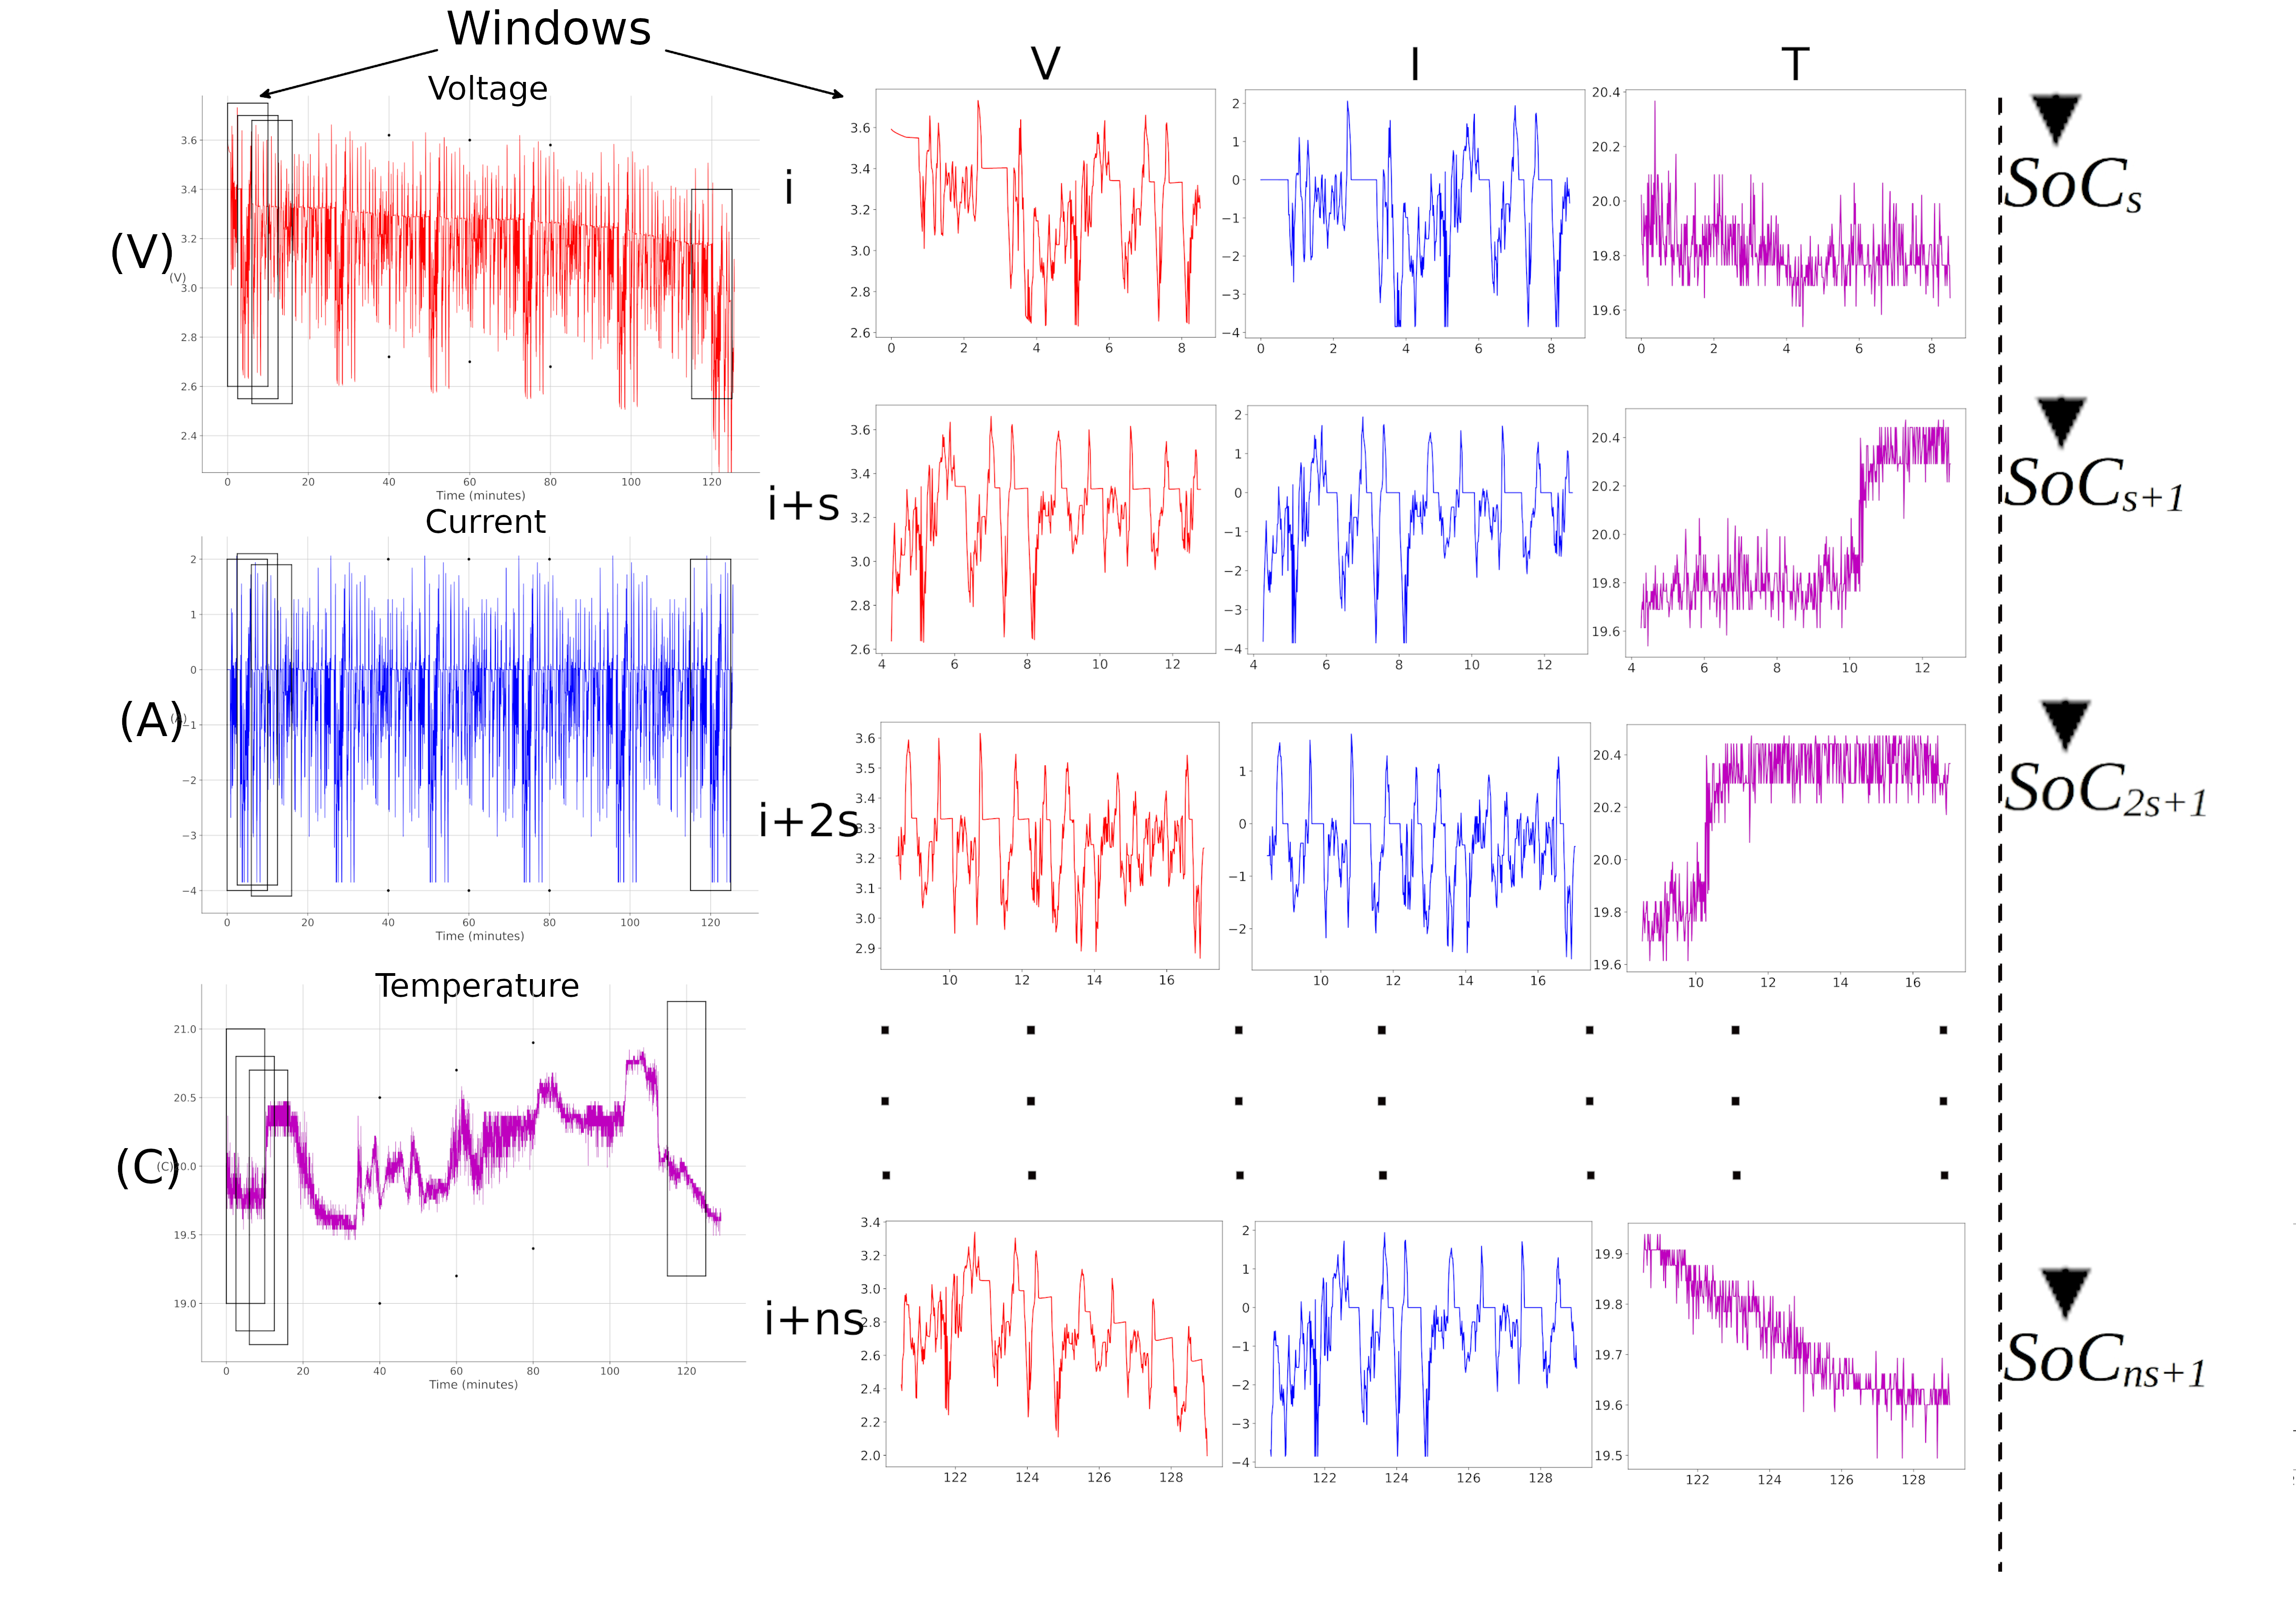
\includegraphics[width=\linewidth]{II_Body/images/windowing3f-A3.jpg}
        \caption{Data Windowing scheme. For visualisation purposes, the $s$-step has been used as 250 seconds, which is different from actual implementation. Initial index $i$ was kept as a value close to the beginning of the data, around zero.}
        \label{fig:Windowing3f}
    \end{figure}
\end{landscape}